\documentclass{my_paper}
\usepackage{ctex}
\usepackage[textwidth=444bp,vmargin=2.5cm]{geometry}%设置页边距
\usepackage{array} %主要是增加列样式选项
\usepackage[dvipsnames]{xcolor}%颜色宏包
\usepackage{graphicx}%图片宏包
\usepackage{amsmath}%公式宏包
\usepackage[T1]{fontenc}    
\usepackage{newtxtext, newtxmath}  %两种使用Times New Roman 字体的方法
\usepackage{subfigure}
\usepackage{tabularx, booktabs} %% Load packages that you use
\usepackage{multirow} %跨行处理
\usepackage{rotating}%横向表格
\usepackage{diagbox}%斜线划分表头

\usepackage { gensymb }
% 打°符号\degree
\usepackage{framed}
\usepackage{listings}
% 代码
\usepackage{color} %red, green, blue, yellow, cyan, magenta, black, white
\usepackage[numbered,framed]{matlab-prettifier}%matlab 代码高亮
\usepackage{mdframed}%另一个边框
% matlab代码样式,使用方法为:
% \lstinputlisting[style=Matlab-editor,linewidth=\textwidth]{code.m}
% 或:
% \begin{lstlisting}[style=matlab-prettifier]
%     %code
% \end{lstlisting}
\renewenvironment{framed}[1][\hsize]
  {\MakeFramed{\hsize#1\advance\hsize-\width \FrameRestore}}%
  {\endMakeFramed}
%   修正framed环境,使之可以变长,用法:
%   \begin{framed}[1.2/textwidth]...

\usepackage{hologo}
\usepackage{gbt7714}
\bibliographystyle{gbt7714-numerical}
% 采用国标参考文献引用
\newcommand{\lunwenbiaoti}{\fontsize{15.75pt}{0}\heiti 基于PID自动控制的暖气房屋控温模型}
\newcommand{\zhaiyao}{\fontsize{14pt}{0}\heiti 摘要}
    
\begin{document}

\lstdefinestyle{python_style}{
 columns=fixed,
 numbers=left,                                        % 在左侧显示行号
 numberstyle=\tiny\color{gray},                       % 设定行号格式
 frame=trbl,                                        % 单线背景边框
 breaklines=true,                                     % 设定LaTeX对过长的代码行进行自动换行
 keywordstyle=\color[RGB]{40,40,255},                 % 设定关键字颜色
 numberstyle=\footnotesize\color{darkgray},
 commentstyle=\it\color[RGB]{0,96,96},                % 设置代码注释的格式
 stringstyle=\rmfamily\slshape\color[RGB]{128,0,0},   % 设置字符串格式
 showstringspaces=false,                              % 不显示字符串中的空格
 language=python,                                        % 设置语言
 basicstyle=\linespread{1.0}\fontsize{10bp}{10bp}\selectfont\ttfamily,                      % 字体字号
 %lineskip=10bp,
 %baselinestretch=1,
}
\newpage
\begin{center}
\lunwenbiaoti

\vspace{2ex}
\zhaiyao
\end{center}

摘要

\begin{guanjianci}
 元胞自动机 \quad 边缘检测 \quad 形状匹配
\end{guanjianci}

%----------- 正文 ----------
%----------- 一、问题重述 ----------
\newpage
\section{一、问题重述}

\subsection{问题背景}

一企业使用A、B、C三种可相互替代的原料生产某种建筑和装饰板材。在生产过程中,需要及时向供应商订购物资,并且指派转运商进行转运。由于原材料的特殊性,供应商
不能保证严格按订货量供货,实际供货量可能多于或少于订货量。且转运商在转运过程中可能导致原材料的损耗,不同的转运商具有不同的损耗率。

为了维持生产所需,企业应该尽量保持不少于两周的生产备货量,在这一系列条件下,我们需要基于材料所给数据,制定企业调度供应商以及转运商的策略。

\subsection{问题重述}
经过分析整理,我们需要解决以下问题:
\begin{enumerate}
    \item 对402家供应商的订货以及供货情况进行分析,建立保障企业生产重要性的数学模型,在所给的供应商中选出50个最重要的供应商,在论文中列出结果。
    \item 在问题一的基础上,估计满足企业生产需求所需的供应商数目,对于这些供应商而言,制定最经济的订购方案以及损耗最少的转运方案,以指定格式输出到附件中。
    \item 为了压缩企业的仓储成本,计划尽量多的采购A类原材料和尽量少的采购C类原材料,同时希望企业的转运损耗尽可能小。就此确定新的采购方案,并且分析新采购方案的实施效果。
    \item 若企业经过技术改造后,具有提高产能的潜力,根据供应商和转运商的实际情况,确定每周的产能提高情况,并给出订购和转运的方案。
\end{enumerate}
\section{二、问题分析}
\subsection{问题一的分析}

针对问题一,需要确定402家供应商中最重要的50家。为此,需要由附件中的企业订货数量和供应商的供货量之间的关系进行判断。由于供货的特殊性,供货与订货数量不能完全保持一致,若供货不及时,可能带来原料缺口,影响企业的生产过程。

与此同时,不同供应商之间的供应能力也有较大差异,部分供应商倾向于连续供货,而部分倾向于集中供货。我们需要将指标量化后,综合赋予权重,对每家供应商进行打分,最终比较出最重要的50家供应商。

\subsection{问题二的分析}

分析

\subsection{问题三的分析}


%----------- 三、模型假设 ----------
\section{三、模型假设}
%使用代码片段:、jiashe%
\begin{enumerate}
    \item 
    
    \textbf{原因:}


\end{enumerate}

%----------- 四、符号说明 ----------
\section{四、名词解释与符号说明}
%使用三线表格最好~
\subsection{名词解释}
\begin{enumerate}
    % 名词:、mingci
    \item \textbf{dada}
    
    dsadw
    
    \item \textbf{dsadc}
    
    dasdsas

    
\end{enumerate}
\subsection{符号说明}
以下是本文使用的符号以及含义:
\begin{table}[h]%htbp表示的意思是latex会尽量满足排在前面的浮动格式,就是h-t-b-p这个顺序,让排版的效果尽量好。
    \centering
    \begin{tabular}{p{2.0cm}<{\centering}p{9.0cm}<{\centering}p{2.0cm}<{\centering}}
 %指定单元格宽度, 并且水平居中。
    \hline
    符号 & 说明 & 单位 \\ %换行 
    \hline
    $L_0$ & 仓库长度 &  $m$\\
    
    \hline
    \end{tabular}
\end{table}

%----------- 五、模型的建立与求解 ----------
\section{五、模型的建立与求解}

以下将对提出的四个问题进行建模求解。

\subsection{重要供应商筛选模型}
为了能够筛选出重要的供应商,我们提出了一种基于熵权法的打分模型,以履约执行性、供货稳定性、供货产能、签约存续性和库存持续性五个指标作为评判标准。最终筛选出50家重要的供应商。
\subsubsection{模型建立}
经过分析和思考,我们列出五个反应供应商情况的重要指标,综合了每周和长期的订单交付情况。这五个指标综合反映了供应商的特点,较为全面综合了局部与全局的信息。

\begin{enumerate}
    \item 履约执行性 $a_1$
    
    在供应链管理的过程中,风险管理\cite{1}是非常重要的环节,事关企业的生产计划能否按需完成。在题目的条件中,我们不能获悉供应商的财务报表、人事构成等情况,但是可以通过企业的订货量$R$和供应商的供货量$S$之间的关系来分析企业的履约情况,也就是履约执行性$a_1$。该指标判断了供应商在有订单的条件下,执行订单的总体情况。要量化计算履约执行性,我们首先需要引入两个指标:订单空白$b_{ij}$和供求评分$c_{ij}$。订单空白是个二值变量,用于标记某供应商在某周是否有订单;供求评分$c_{ij}$是一个分段函数,用于量化估计供应与订单量的相对大小。二者的计算公式如下所示:
    \begin{equation}
    b_{ij} = \begin{cases}
        0&,R_{ij}=0\\
        1&,R_{ij}\neq 0\\
    \end{cases}
    \label{bij}
    \end{equation}
    \begin{equation}
    c_{ij}=\begin{cases}
        0,&R_{ij}>S_{ij}\\
        1,&R_{ij}=S_{ij}\\
        0.8,&R_{ij}<S_{ij}\\
    \end{cases}
    \label{cij}
    \end{equation}
    ,其中$R$和$S$分别代表企业的订货量和供应商的供货量。上述公式中$i$代表周数,$j$代表供应商的编号,下同。
    
    $c$的意义在于判断订单的执行情况,最理想的条件下,企业发出订单,在一周内供应商能够按约定量交付,则此时量化评分为1;若供应商不能够按约执行的话,分为两种情况进行考虑:一种是供大于求,此时虽然没有按约执行,但是充实了企业的备用库存,结果不算差,故量化评分为$0.8$。另一种是供不应求,此时企业消耗库存以填补原料缺口,可能导致库存消耗甚至是影响产量的问题。
    
    在得到两个中间变量后,便可给出履约情况的计算式:
    \begin{equation}
    a_{j1}=\frac{\sum\limits^n_{i=1}c_{ij}}{\sum\limits^n_{i=1}b_{ij}}
    \label{aj1}
    \end{equation}
    ,其中$n$为附件数据中所给的周数。$a_i$的意义在于量化统计供应商在每周内的履约情况。对于那些没有在一周内按数量交付的供应商,该评分的数值较低,而如果一家供应商能够准时供货,则该指标数值就较大。

    \item 供货稳定性 $a_2$
    
    选取两个供应商的每周供货情况,绘制成折线图,如图(\ref{11})所示。
    \begin{figure}[htbp]
        \centering  %居中
        \subfigure[S005]{   %第一张子图
        \begin{minipage}{\textwidth}%大小总和超过textwidth则自动换行
        \centering    %子图居中
        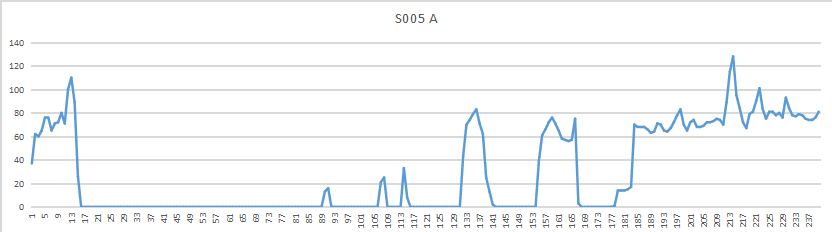
\includegraphics[width=\textwidth]{11005.png}  %设置图片的输出大小倍数,这里是0.5倍大小输出
        \end{minipage}
        }\\
        \subfigure[S007]{ %第二张子图
        \begin{minipage}{\textwidth}
        \centering    %子图居中
        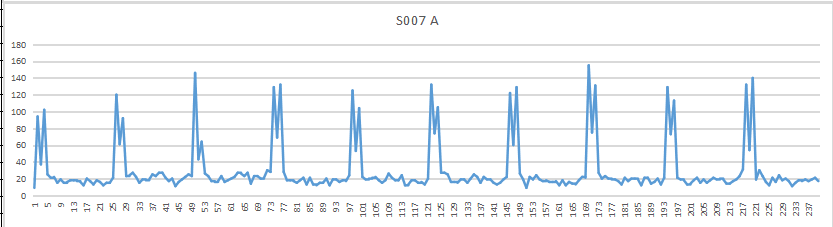
\includegraphics[width=\textwidth]{11007.png}%以pic.jpg的0.5倍大小输出
        \end{minipage}
        }
        注:横轴为周数单位为周,纵轴为供货量单位为$m^3$
    
        \caption{不同供应商的供货情况}    %大图名称
        \label{11}    %图片引用标记
    \end{figure}
    \newpage
    可见供应商由于各种原因,可能不具有连续供应的能力,导致一段时间内企业不能收到原材料。为此,提出供货稳定性这一指标$a_2$,用于统计供应商能够连续供货的情况。其计算方法为统计订单和供货量均大于0的最大连续天数$d$,计算方法如下:
    \begin{equation}
    d_i = \begin{cases}
        d_{i-1}+1,&R_i>0 \quad\&\quad S_i>0\\
        0, & else
    \end{cases}
    \label{d}
    \end{equation}
    ,其中$d_0=0$,对序列进行计算后,令其中的最大值为$a_2$,即:
    \begin{equation}
    a_2=\underset{i}{argmax}\quad d_{ij}
    \label{a2}
    \end{equation}
    对于供应商而言,具有较高的$a_2$数值意味着具有更好的连续供货的能力,以满足连续的生产需求,更有利于判断其生产的规律性。而具有较低数值的企业可能会有较大供应波动,导致不合理的订货情况。

    \item 供货产能 $a_3$
    
    观察附件中数据可知,不同供应商之间的供应能力也有较大差异,表现在每周的供货数量的平均值上有一定区别。之所以不使用最大值来评估供货商的供应能力,是因为某天内供应商的大量出货可能是由于订单数目的增多,不能够全面反映出供应商的原料出产水平。此外,供应商可能会提供A、B、C三种原料中的一种,不同原料的出品率有所不同,因此需要衡量企业最终产出的数量。考虑到企业每周的生产量达到了万立方米级别,因此供应商的产量不能太低,否则导致调度配合过程中成本上升。综合上述分析,提出供货产能$a_3$的计算方法:
    \begin{equation}
    a_{j3}=\frac{\sum\limits^n_{i=1} S_i}{n}\cdot \alpha
    \label{aj3}
    \end{equation}
    ,$\alpha$是产出系数,同原料种类$M$的不同而变化:
    $$\alpha=\begin{cases}
        \frac{1}{0.6} ,& M=A\\
        \frac{1}{0.66} ,& M=B\\
        \frac{1}{0.72} ,& M=C\\
    \end{cases}$$

    \item 签约存续性 $a_4$
    
    在历史的订单数据中,企业已经同供应商合作240周的时间,这段时间中供应商若能同企业配合良好,企业便有更高的概率向这一企业订购材料;而反之若双方合作不愉快,企业便不愿意再订购,长期上看便是具有较少的交货量。经过上述分析,给出签约存续性$a_{4}$的计算式:
    \begin{equation}
    a_{j4}=\frac{\sum\limits^n_{i=1}b_{ij}}{n}
    \label{aj4}
    \end{equation}
    ,其中$b_{ij}$已经由式(\ref{bij})给出,表示的是某周是否交付原料。

    \item 库存持续性 $a_5$
    
    如背景中所述,企业在规划生产活动时,会预留两周的原料储备,以应对不能即使供应的情况,这部分库存常被称作是安全库存\cite{1}。安全库存的概念是就企业整体的生产而言,但是我们可以就整体和局部的关系来看,如果企业的每个供应商都能够保证订单交付的情况能满足安全库存,则企业的安全库存无虞。
    
    在这一前提条件下,我们认为企业向某个供应商定下的订单是基于库存和生产需求来确定的,若某周供应商的库存不能满足未来两周的订单要求,则认为是“缺口周”。以附件一中S66供应商W001-W006的数据来分析可得下表:
    \begin{table}[ht]

    \centering
    \caption{以S66供应商为例分析缺口周情况表}
    \begin{tabular}{c|ccccccc}
    \toprule
    周数      & W001 & W002 & W003 & W004 & W005 & W005 & W006 \\\midrule
订货量     & 1    & 0    & 1    & 0    & 0    & 0    & 3    \\
供货量     & 2    & 0    & 1    & 0    & 0    & 0    & 4    \\
仓库剩余原料量 & 1    & 1    & 1    & 1    & 1    & 1    & 2    \\
未来两周订货量 & 1    & 1    & 0    & 0    & 3    & 3    & 3    \\
是否为缺口   & 否    & 否    & 否    & 否    & 是    & 是    & 是\\
    \bottomrule
      \end{tabular}
    
    \label{label}
      \end{table}
    
    我们提出的库存持续性$a_5$这一指标即统计了缺口时长。首先以递归形式给出原料库存$h$的计算公式:
    \begin{equation}
    h_i=h_{i-1}+R_i-S_i
    \label{hi}
    \end{equation}
    ,其中$h_0=0$,只需遍历订单和供应量列表即可获得库存的情况,在此基础上判断与未来两周的需求可以统计出$a_5$:
    \begin{equation}
    a_5 = |\{ h_{ij} |\forall 1\leq i \leq n-2 \quad h_{ij}\geq R_{i+1,j}+R_{i+2,j}\}|
    \label{aj5}
    \end{equation}
    
\end{enumerate}

在分析总结出履约执行性、供货稳定性、供货产能、签约存续性和库存持续性这五个重要的因素之后,需要对这些因素进行归一化处理,以判断其相对的重要程度。在众多方法如AHP主成分分析法\cite{2},熵权法\cite{3},主观赋权法之间,我们使用熵权法来衡量指标之间的重要程度。由于上述五个指标量纲不一致,需要对数据进行归一化处理,计算式如下:
\begin{equation}
a_{ij}=\frac{a_{ij}-min(a_i)}{max(a_i)-min(a_i)}
\label{aij}
\end{equation}

在归一化之后,使用熵权法计算各个指标应当配比的权重,其基本思想是根据指标的变化幅度来赋予权重。熵权法的计算过程如下所示:

\subsubsection{模型求解}
\section{六、敏感性分析}
\section{七、模型的评价}

\subsection{模型的优点}
\begin{enumerate}
    \item 采用

\end{enumerate}

\subsection{模型的缺点}
\begin{itemize}
    \item 利用较

\end{itemize}

%----------- 参考文献 ----------
\newpage
\begin{center}
\bibliography{reference} %调出LaTeX生成参考文献列表
\end{center}

%----------- 附录 ----------
\newpage
\section{附件}
\textbf{附件清单:}
\renewcommand\theenumi{\roman{enumi}}
% 规定数字格式为罗马数字
\renewcommand\labelenumi{\textbf{附录\theenumi}}
% 规定是附录某某
\begin{itemize}
    \item xxx代码
\end{itemize}

\textbf{sobel边缘检测代码}

\begin{lstlisting}[language=matlab]
    function GAdsa 
\end{lstlisting}



\end{document}